\input{si.tex}



\section*{S1 Text : Extended Figures for Model Exploration}


\subsection*{Convergence}

Histograms for the 81 parameters points for which we did 100 repetitions are given in Fig.~\ref{fig:histograms}, for Moran index and slope indicators. Other indicators showed similar convergence patterns. The visual exploration of histograms confirms the numerical analysis done in main text for statistical convergence.

% histograms


% and bimodal statistical distribution for cumulated points in the parameter space confirm the existence of superposed regimes : gaussian distribution gives stationary configurations, whereas inverse log-normal distribution are close to real data shape and correspond to non-stationary regime.
% -> not sure it is interesting to look at cumulated histograms.

% Figures :

%%%%%%%%%%%%%%%%%%%%
\begin{figure}
\centering
\includegraphics[width=\textwidth]{figuresraw/hist_moran}\\
\includegraphics[width=\textwidth]{figuresraw/hist_slope}
\caption{Histograms for Moran index (top) and slope (bottom), for varying $\alpha$ (columns), $\beta$ (rows), $N_G$ and $n_d$ (colors).}
\label{fig:histograms}
\end{figure}
%%%%%%%%%%%%%%%%%%%%







\subsection*{Indicators Behavior}

% full plots behavior

We show in Fig.2 to Fig.5 the full behavior of all indicators, with all parameters varying, obtained through the extensive exploration, from which the plots in main text have been extracted. Because of the complex nature of emergent urban form, one can not predict output values without referring to this ``exhaustive'' parameter sweep.


%%%%%%%%%%%%%%%%%%%%
\begin{figure}
\centering
\includegraphics[width=\textwidth]{figuresraw/moran_alpha}
\includegraphics[width=\textwidth]{figuresraw/moran_beta}
\caption{Moran index as a function of $\alpha$ (Top) and $\beta$ (Bottom) for varying $\beta$ (resp. $\alpha$) given by color, and varying $n_d$ (rows) and $N_G$ (columns).}
\label{fig:moran}
\end{figure}
%%%%%%%%%%%%%%%%%%%%

%%%%%%%%%%%%%%%%%%%%
\begin{figure}
\centering
\includegraphics[width=\textwidth]{figuresraw/slope_alpha}
\includegraphics[width=\textwidth]{figuresraw/slope_beta}
\caption{Slope as a function of $\alpha$ (Top) and $\beta$ (Bottom) for varying $\beta$ (resp. $\alpha$) given by color, and varying $n_d$ (rows) and $N_G$ (columns).}
\label{fig:slope}
\end{figure}
%%%%%%%%%%%%%%%%%%%%


%%%%%%%%%%%%%%%%%%%%
\begin{figure}
\centering
\includegraphics[width=\textwidth]{figuresraw/distance_alpha}
\includegraphics[width=\textwidth]{figuresraw/distance_beta}
\caption{Average distance index as a function of $\alpha$ (Top) and $\beta$ (Bottom) for varying $\beta$ (resp. $\alpha$) given by color, and varying $n_d$ (rows) and $N_G$ (columns).}
\label{}
\end{figure}
%%%%%%%%%%%%%%%%%%%%

%%%%%%%%%%%%%%%%%%%%
\begin{figure}
\centering
\includegraphics[width=\textwidth]{figuresraw/entropy_alpha}
\includegraphics[width=\textwidth]{figuresraw/entropy_beta}
\caption{Entropy as a function of $\alpha$ (Top) and $\beta$ (Bottom) for varying $\beta$ (resp. $\alpha$) given by color, and varying $n_d$ (rows) and $N_G$ (columns).}
\label{}
\end{figure}
%%%%%%%%%%%%%%%%%%%%




\subsection*{Indicators Scatterplots}

% scatterplots - with real points

We show finally the full scatterplots of indicators, with real data points, in Fig.~\ref{fig:densityscatter}. These are preliminary step of the calibration on principal components, and we can see on these on which dimensions the model fails relatively to fit real data (in particular average distance).


%%%%%%%%%%%%%
\begin{figure}
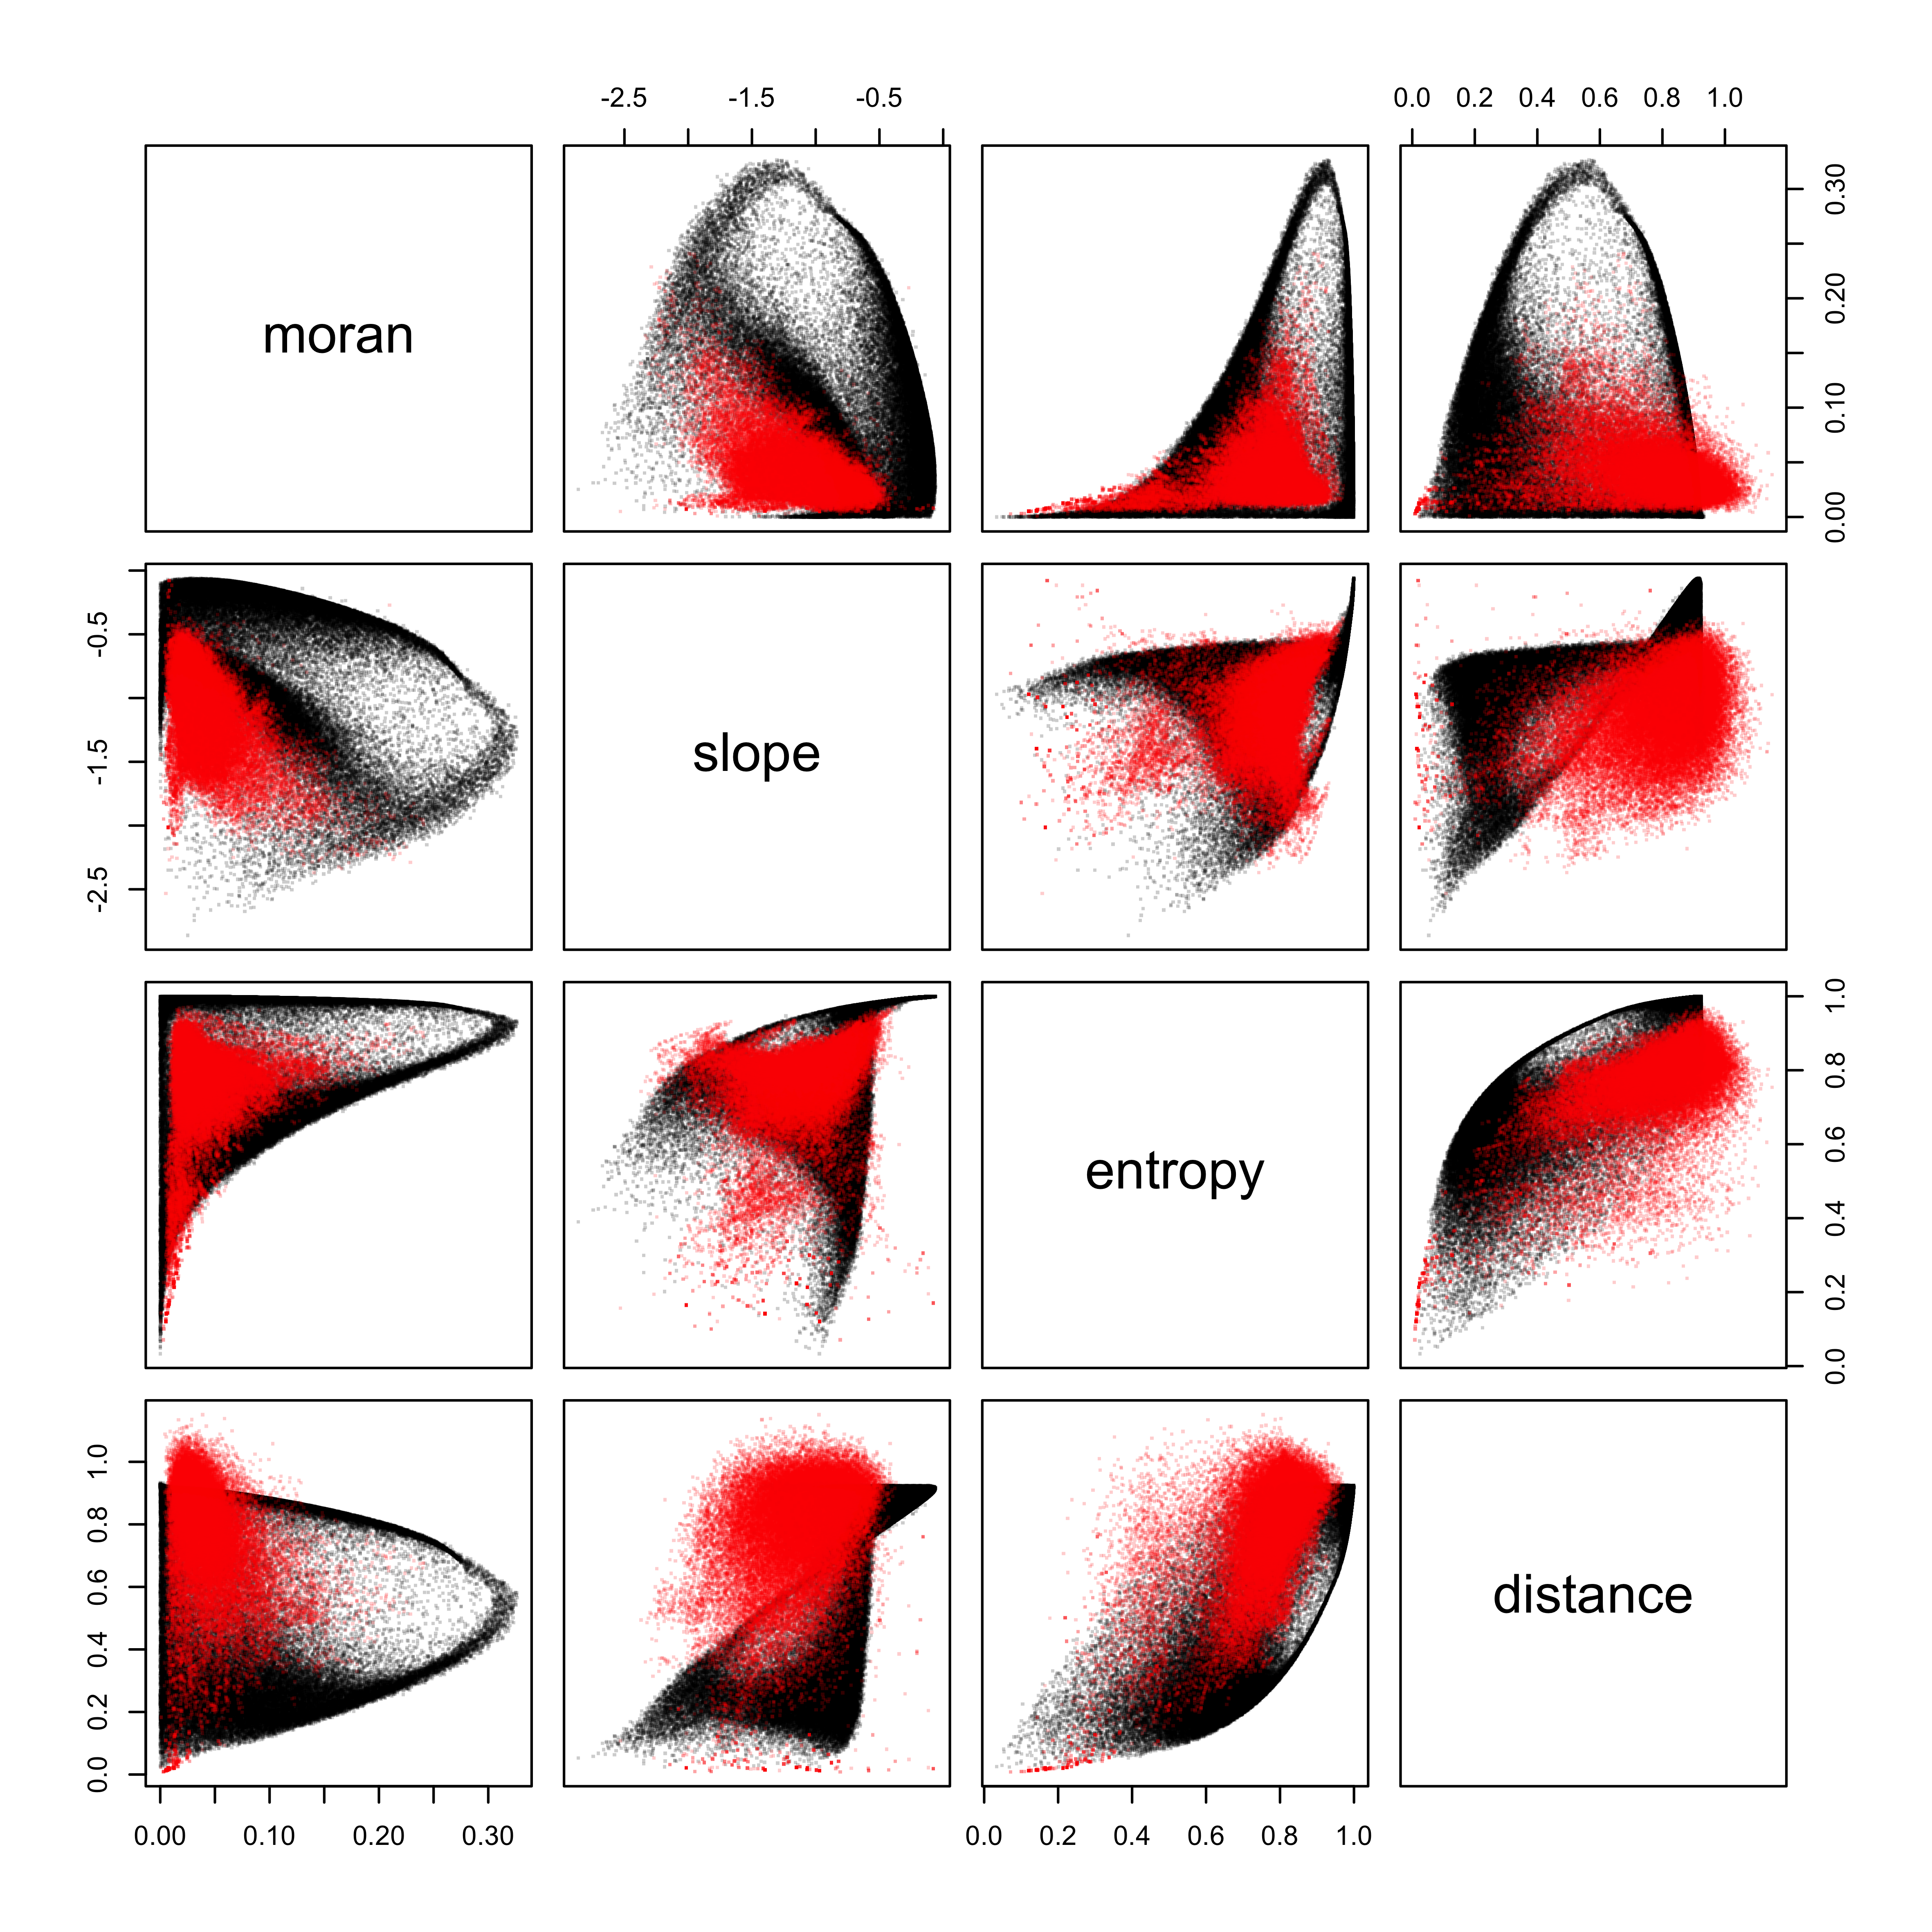
\includegraphics[width=\textwidth]{figuresraw/scatter}
\caption{Scatterplots of indicators distribution in the sampled hypercube of the parameter space. Red points correspond to real data.}
\label{fig:densityscatter}
\end{figure}
%%%%%%%%%%%%%






\end{document}
